% Options for packages loaded elsewhere
\PassOptionsToPackage{unicode}{hyperref}
\PassOptionsToPackage{hyphens}{url}
\documentclass[
  11pt,
]{article}
\usepackage{xcolor}
\usepackage[margin=1in]{geometry}
\usepackage{amsmath,amssymb}
\setcounter{secnumdepth}{-\maxdimen} % remove section numbering
\usepackage{iftex}
\ifPDFTeX
  \usepackage[T1]{fontenc}
  \usepackage[utf8]{inputenc}
  \usepackage{textcomp} % provide euro and other symbols
\else % if luatex or xetex
  \usepackage{unicode-math} % this also loads fontspec
  \defaultfontfeatures{Scale=MatchLowercase}
  \defaultfontfeatures[\rmfamily]{Ligatures=TeX,Scale=1}
\fi
\usepackage[]{libertine}
\ifPDFTeX\else
  % xetex/luatex font selection
\fi
% Use upquote if available, for straight quotes in verbatim environments
\IfFileExists{upquote.sty}{\usepackage{upquote}}{}
\IfFileExists{microtype.sty}{% use microtype if available
  \usepackage[]{microtype}
  \UseMicrotypeSet[protrusion]{basicmath} % disable protrusion for tt fonts
}{}
\makeatletter
\@ifundefined{KOMAClassName}{% if non-KOMA class
  \IfFileExists{parskip.sty}{%
    \usepackage{parskip}
  }{% else
    \setlength{\parindent}{0pt}
    \setlength{\parskip}{6pt plus 2pt minus 1pt}}
}{% if KOMA class
  \KOMAoptions{parskip=half}}
\makeatother
\usepackage{color}
\usepackage{fancyvrb}
\newcommand{\VerbBar}{|}
\newcommand{\VERB}{\Verb[commandchars=\\\{\}]}
\DefineVerbatimEnvironment{Highlighting}{Verbatim}{commandchars=\\\{\}}
% Add ',fontsize=\small' for more characters per line
\usepackage{framed}
\definecolor{shadecolor}{RGB}{248,248,248}
\newenvironment{Shaded}{\begin{snugshade}}{\end{snugshade}}
\newcommand{\AlertTok}[1]{\textcolor[rgb]{0.94,0.16,0.16}{#1}}
\newcommand{\AnnotationTok}[1]{\textcolor[rgb]{0.56,0.35,0.01}{\textbf{\textit{#1}}}}
\newcommand{\AttributeTok}[1]{\textcolor[rgb]{0.13,0.29,0.53}{#1}}
\newcommand{\BaseNTok}[1]{\textcolor[rgb]{0.00,0.00,0.81}{#1}}
\newcommand{\BuiltInTok}[1]{#1}
\newcommand{\CharTok}[1]{\textcolor[rgb]{0.31,0.60,0.02}{#1}}
\newcommand{\CommentTok}[1]{\textcolor[rgb]{0.56,0.35,0.01}{\textit{#1}}}
\newcommand{\CommentVarTok}[1]{\textcolor[rgb]{0.56,0.35,0.01}{\textbf{\textit{#1}}}}
\newcommand{\ConstantTok}[1]{\textcolor[rgb]{0.56,0.35,0.01}{#1}}
\newcommand{\ControlFlowTok}[1]{\textcolor[rgb]{0.13,0.29,0.53}{\textbf{#1}}}
\newcommand{\DataTypeTok}[1]{\textcolor[rgb]{0.13,0.29,0.53}{#1}}
\newcommand{\DecValTok}[1]{\textcolor[rgb]{0.00,0.00,0.81}{#1}}
\newcommand{\DocumentationTok}[1]{\textcolor[rgb]{0.56,0.35,0.01}{\textbf{\textit{#1}}}}
\newcommand{\ErrorTok}[1]{\textcolor[rgb]{0.64,0.00,0.00}{\textbf{#1}}}
\newcommand{\ExtensionTok}[1]{#1}
\newcommand{\FloatTok}[1]{\textcolor[rgb]{0.00,0.00,0.81}{#1}}
\newcommand{\FunctionTok}[1]{\textcolor[rgb]{0.13,0.29,0.53}{\textbf{#1}}}
\newcommand{\ImportTok}[1]{#1}
\newcommand{\InformationTok}[1]{\textcolor[rgb]{0.56,0.35,0.01}{\textbf{\textit{#1}}}}
\newcommand{\KeywordTok}[1]{\textcolor[rgb]{0.13,0.29,0.53}{\textbf{#1}}}
\newcommand{\NormalTok}[1]{#1}
\newcommand{\OperatorTok}[1]{\textcolor[rgb]{0.81,0.36,0.00}{\textbf{#1}}}
\newcommand{\OtherTok}[1]{\textcolor[rgb]{0.56,0.35,0.01}{#1}}
\newcommand{\PreprocessorTok}[1]{\textcolor[rgb]{0.56,0.35,0.01}{\textit{#1}}}
\newcommand{\RegionMarkerTok}[1]{#1}
\newcommand{\SpecialCharTok}[1]{\textcolor[rgb]{0.81,0.36,0.00}{\textbf{#1}}}
\newcommand{\SpecialStringTok}[1]{\textcolor[rgb]{0.31,0.60,0.02}{#1}}
\newcommand{\StringTok}[1]{\textcolor[rgb]{0.31,0.60,0.02}{#1}}
\newcommand{\VariableTok}[1]{\textcolor[rgb]{0.00,0.00,0.00}{#1}}
\newcommand{\VerbatimStringTok}[1]{\textcolor[rgb]{0.31,0.60,0.02}{#1}}
\newcommand{\WarningTok}[1]{\textcolor[rgb]{0.56,0.35,0.01}{\textbf{\textit{#1}}}}
\usepackage{graphicx}
\makeatletter
\newsavebox\pandoc@box
\newcommand*\pandocbounded[1]{% scales image to fit in text height/width
  \sbox\pandoc@box{#1}%
  \Gscale@div\@tempa{\textheight}{\dimexpr\ht\pandoc@box+\dp\pandoc@box\relax}%
  \Gscale@div\@tempb{\linewidth}{\wd\pandoc@box}%
  \ifdim\@tempb\p@<\@tempa\p@\let\@tempa\@tempb\fi% select the smaller of both
  \ifdim\@tempa\p@<\p@\scalebox{\@tempa}{\usebox\pandoc@box}%
  \else\usebox{\pandoc@box}%
  \fi%
}
% Set default figure placement to htbp
\def\fps@figure{htbp}
\makeatother
\setlength{\emergencystretch}{3em} % prevent overfull lines
\providecommand{\tightlist}{%
  \setlength{\itemsep}{0pt}\setlength{\parskip}{0pt}}
\usepackage[]{natbib}
\bibliographystyle{apsr}
\usepackage{hyperref}
\usepackage{array}
\usepackage{caption}
\usepackage{graphicx}
\usepackage{siunitx}
\usepackage[table]{xcolor}
\usepackage{multirow}
\usepackage{hhline}
\usepackage{calc}
\usepackage{tabularx}
\usepackage{fontawesome}
\usepackage[para,online,flushleft]{threeparttable}
\usepackage{wrapfig}
\captionsetup[wrapfigure]{justification=raggedright,singlelinecheck=false}
\usepackage{bookmark}
\IfFileExists{xurl.sty}{\usepackage{xurl}}{} % add URL line breaks if available
\urlstyle{same}
\hypersetup{
  pdftitle={Introduction to R \& RStudio},
  pdfauthor={Data Science for the Psychological Sciences},
  pdfkeywords={r, r markdown},
  hidelinks,
  pdfcreator={LaTeX via pandoc}}

\title{Introduction to R \& RStudio}
\author{Data Science for the Psychological Sciences}
\date{}

\begin{document}
\maketitle

\section{What is R?}\label{what-is-r}

R is a free, open-source programming environment designed for
statistical computing, data analysis, and scientific visualization. It
combines an interactive console for exploratory work with a rich
ecosystem of packages that support everything from data cleaning and
modeling to reproducible reporting and interactive applications. In the
R environment, users typically write scripts that import and transform
data, generate graphics, and fit statistical or machine learning models,
with results that can be documented and shared through tools such as R
Markdown and Quarto. Because R is widely used in research and industry
and is especially strong for statistical methodology and high-quality
plotting, it is a practical platform for psychologists and other social
scientists who need transparent, replicable workflows for analyzing data
and communicating findings.

\emph{Unit goals:}

\begin{enumerate}
\def\labelenumi{\arabic{enumi}.}
\tightlist
\item
  Introduce the RStudio integrated development environment (IDE).
\item
  To provide a hands-on introduction to the R programming environment.
\end{enumerate}

\section{RStudio/Rmarkdown}\label{rstudiormarkdown}

\begin{wrapfigure}{r}{0.40\textwidth}
  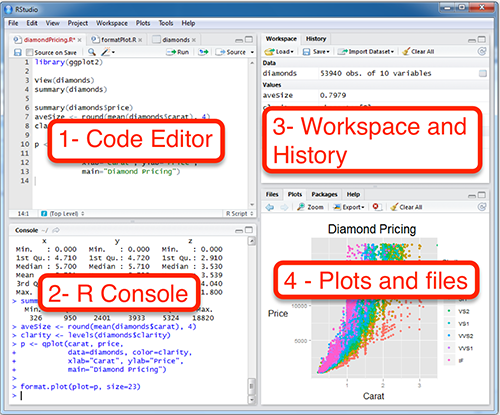
\includegraphics[width=0.38\textwidth]{rstudio.png}
  \caption{RStudio interface.}
  \label{fig:rstudio}
\end{wrapfigure}

R is a standalone application, meaning that it can be installed and used
as-is, but both learning and using R can be facilitated by combining it
with an integrated development environment (IDE) like Jupyter Notebooks,
Rcommander, or Rstudio (just to name a few).

In this class, you will be using RStudio, an integrated development
environment (IDE) for the R programming language that makes it easier to
write code, manage files, and run analyses in one place. RStudio
provides a clear interface for working with scripts, viewing data,
creating plots, and installing and using packages, which supports an
efficient and reproducible workflow. Over the course of the term, you
will use RStudio to import and clean data, generate visualizations, and
conduct statistical and machine learning analyses, while documenting
your work in a way that can be shared and revisited (see Figure
\ref{fig:rstudio}).

An advantage of using RStudio is that it permits the seamless
integration of text, code, and output within a single, coherent
workflow, which is especially valuable for producing transparent and
reproducible analyses. By combining narrative explanation with
executable R code, tables, and figures, you can document not only what
results you obtained, but also exactly how you obtained them---making
your work easier to verify, update, and share. This approach supports
best practices in modern data science and psychological research, where
the goal is to move from ad hoc analyses to well-organized projects that
can be rerun end-to-end as data or research questions evolve.

\subsection{R Markdown Formatting
Basics}\label{r-markdown-formatting-basics}

RStudio supports writing and analysis through R Markdown, a format that
lets you combine plain-language text with executable R code in a single
document that can be rendered into polished outputs such as HTML, PDF,
or Word. This ``literate programming'' approach is valuable because it
keeps your narrative, analysis, and results together, reducing the risk
of copy-and-paste errors and making it straightforward to reproduce your
work later. In practice, R Markdown encourages a clean, transparent
workflow: you write what you are doing and why, run the code that
performs the analysis, and generate figures and tables directly from the
underlying data---so the final document can be regenerated whenever
inputs change, rather than manually rebuilt. R Markdown allows you to
create beautifully formatted documents, uses a simple syntax to create
headers, lists, links, and more.

\subsubsection{R Code Chunks}\label{r-code-chunks}

As you'll see throughout this document, R code is placed in ``chunks,''
which are clearly marked sections of an R Markdown file that tell
RStudio what to run and what to display in the final output. Each chunk
can contain one or more lines of code, and when you knit the document, R
executes the code and inserts the resulting tables, figures, or printed
output directly into the report. This chunk-based structure helps keep
analyses organized, makes it easier to rerun and troubleshoot specific
steps, and supports reproducibility by ensuring that the results shown
in the document are generated from the code that accompanies them.

You can start a code chunk in an Rmarkdown document using three accent
characters followed by the lowercase letter r in braces and you can end
the code chunk using another set of three accent characters (see example
below). Any R code in between the opening and closing of the code chunk
is executable. Any output from the code execution will appear directly
below the chunk in the final, knitted document.

\texttt{\textasciigrave{}\textasciigrave{}\textasciigrave{}\{r\}}

\texttt{R\ code\ goes\ here}

\texttt{\textasciigrave{}\textasciigrave{}\textasciigrave{}}

The header at the beginning of each chunk, the \texttt{\{r\}}, can
include chunk options/parameters that control how the code is run and
how its output appears in the final document. These options let you
decide whether a chunk should be executed at all (\texttt{eval}),
whether the code itself should be shown to the reader (\texttt{echo}),
and whether messages or warnings should be displayed (\texttt{message},
\texttt{warning}). You can also control how figures are produced and
formatted---for example, providing a figure caption (\texttt{fig.cap}),
adjusting figure size (\texttt{fig.width}, \texttt{fig.height}), setting
the output width (\texttt{out.width}), or specifying where figures
should be placed in a PDF (\texttt{fig.align}). Taken together, chunk
options are a practical tool for creating documents that are both
readable and reproducible: you can keep the analysis code that generates
results while tailoring what the audience sees and how polished the
output looks.

\subsubsection{Headers}\label{headers}

Headers (also called headings) are used to organize your document into
clear sections and subsections, making it easier to read and navigate.
Headers are created with one or more \texttt{\#} symbols at the start of
a line: a single \texttt{\#} typically marks a main section title,
\texttt{\#\#} creates a subsection, and \texttt{\#\#\#} creates a
sub-subsection, with additional \# symbols indicating deeper levels.
Beyond improving readability, headers play a practical role when you
render the document: they can automatically populate a table of
contents, enable section-based navigation in HTML output, and provide a
consistent structure for longer reports, assignments, or manuscripts.
Consistent heading levels also help you communicate the flow of your
analysis---from research question, to methods, to results, to
interpretation---so the narrative and code remain logically connected.

\begin{Shaded}
\begin{Highlighting}[]
\FunctionTok{\#   Level 1 Header}
\FunctionTok{\#\#  Leavel 2 Header}
\FunctionTok{\#\#\# Header 3}
\end{Highlighting}
\end{Shaded}

\subsubsection{Text Emphasis}\label{text-emphasis}

You can make text \emph{italic} or \textbf{bold}.

\begin{itemize}
\tightlist
\item
  \emph{Italic text} is created with \texttt{*asterisks*} or
  \texttt{\_underscores\_}.
\item
  \textbf{Bold text} is created with \texttt{**double\ asterisks**} or
  \texttt{\_\_double\ underscores\_\_}.
\item
  You can even do \textbf{\emph{bold and italic}} with
  \texttt{***triple\ asterisks***}.
\end{itemize}

\subsubsection{Lists}\label{lists}

Lists are a simple way to organize information in R Markdown, whether
you are summarizing key points, outlining steps in an analysis, or
presenting results clearly. Use an unordered (bulleted) list when the
order of items does not matter, and an ordered (numbered) list when you
want to emphasize sequence, ranking, or procedure. You can also create
nested lists by indenting sub-items beneath a main bullet or number,
which is useful for adding detail without cluttering the main flow of
the document.

\emph{Unordered List:}

\begin{Shaded}
\begin{Highlighting}[]
\SpecialStringTok{* }\NormalTok{Item A}
\SpecialStringTok{* }\NormalTok{Item B}
\SpecialStringTok{  * }\NormalTok{Sub{-}item B1}
\SpecialStringTok{  * }\NormalTok{Sub{-}item B2}
\end{Highlighting}
\end{Shaded}

\emph{Ordered List:}

\begin{Shaded}
\begin{Highlighting}[]
\SpecialStringTok{1. }\NormalTok{First item}
\SpecialStringTok{2. }\NormalTok{Second item}
\SpecialStringTok{3. }\NormalTok{Third item}
\end{Highlighting}
\end{Shaded}

\subsubsection{Links and Images}\label{links-and-images}

Links and images are added using straightforward Markdown syntax and are
useful for connecting your document to external resources (e.g.,
documentation, datasets, articles) and for including figures,
screenshots, or diagrams that support your narrative.

Links: Create a hyperlink with \texttt{{[}display\ text{]}(URL)}. For
example: \href{https:www.r.com}{The R Project}. Be sure to choose
display text that clearly describes where the link goes (e.g., ``RStudio
Cheatsheet'' rather than ``click here''), especially in instructional
materials.

Images: Embed an image with
\texttt{!{[}alt\ text{]}(path/to/image.png)}. The alt text is a brief
description of the image that improves accessibility and appears if the
image cannot be loaded. Image paths are usually relative to your project
folder (for example, images/rstudio.png), which helps keep your document
portable and easier to share.

If you need to control image size or placement, you can add simple
formatting. For example, you can set a width directly on the Markdown
image using:

\begin{center}
![RStudio interface](rstudio.png)\{width=200px\}
\end{center}

\subsubsection{Blockquotes and Inline
Code}\label{blockquotes-and-inline-code}

Sometimes you also want to refer to code elements directly in your
writing---for example, the name of a dataset, an object you created, or
a function you are asking students to use. In those cases, inline code
helps the reader immediately recognize that the text refers to code. To
format inline code, wrap it in backticks. For example,
\texttt{\textasciigrave{}code\textasciigrave{}} will print as
\texttt{code}. Inline code is especially helpful for clarifying small
but important details such as distinguishing between mean (an object
name) and mean() (a function), or showing argument names like
\texttt{na.rm\ =\ TRUE} exactly as it should be typed.

\begin{quote}
Blockquotes (like this paragraph) are a simple way to visually separate
quoted material or ``callout'' text from the rest of your document. To
create a blockquote, start a line with \textgreater{} and R Markdown
will indent the text and format it differently from the main body. This
is useful for including short quotations, emphasizing definitions, or
adding instructor notes and reminders. You can also create multi-line
blockquotes by placing \textgreater{} at the beginning of each line.
\end{quote}

\begin{quote}
\begin{quote}
You can also use \texttt{\textgreater{}\textgreater{}} to nest
blockquotes (or include lists inside them) when you need more structure.
\end{quote}
\end{quote}

\subsubsection{The YAML Header}\label{the-yaml-header}

At the very top of an R Markdown file, you will need a block of text
surrounded by three dashes:

\texttt{-\/-\/-}

\texttt{title:\ "My\ Document\ Title"}

\texttt{author:\ "Your\ Name"}

\texttt{date:\ "2025-12-29"}

\texttt{output:\ html\_document}

\texttt{-\/-\/-}

This section is called the YAML header. It controls the overall settings
for your document, including the output format, appearance, and optional
features such as a table of contents.

\emph{Common YAML fields:}

\begin{itemize}
\tightlist
\item
  title: The document title displayed at the top of the rendered output
\item
  author: Optional author line
\item
  date: Optional date line (you can remove it)
\item
  output: The format R Markdown will generate (HTML, PDF, Word, etc.)
\end{itemize}

If you do not want the author/date to appear, delete those lines or set
them to blank (empty quote)

\emph{Choosing Output Formats and Options}

\begin{enumerate}
\def\labelenumi{\arabic{enumi}.}
\tightlist
\item
  \textbf{\emph{HTML output (most flexible)}}
\end{enumerate}

\texttt{-\/-\/-}

\texttt{title:\ "Lab\ Report"}

\texttt{output:}

\texttt{html\_document:}

\begin{verbatim}
`toc: true`

`toc_depth: 2`

`number_sections: true`

`theme: readable`
\end{verbatim}

\texttt{-\/-\/-}

What these options do:

\begin{itemize}
\tightlist
\item
  toc: true adds a table of contents
\item
  toc\_depth controls how many header levels appear in the TOC
\item
  number\_sections automatically numbers headers
\item
  theme changes the visual style of the HTML output
\end{itemize}

\begin{enumerate}
\def\labelenumi{\arabic{enumi}.}
\setcounter{enumi}{1}
\tightlist
\item
  \textbf{\emph{PDF output (print-friendly, more strict formatting)}}
\end{enumerate}

\texttt{-\/-\/-}

\texttt{title:\ "Lab\ Report"}

\texttt{output:}

\texttt{pdf\_document:}

\texttt{toc:\ true}

\texttt{number\_sections:\ true}

\texttt{-\/-\/-}

Note: PDF output requires a LaTeX installation. If you get LaTeX errors,
you may need to install TinyTeX.

\begin{enumerate}
\def\labelenumi{\arabic{enumi}.}
\setcounter{enumi}{2}
\tightlist
\item
  \textbf{\emph{Word output (useful for submissions)}}
\end{enumerate}

\texttt{-\/-\/-}

\texttt{title:\ "Lab\ Report"}

\texttt{output:}

\texttt{word\_document:}

\texttt{toc:\ true}

\texttt{-\/-\/-}

\section{Introduction to R}\label{introduction-to-r}

R's real power comes from the availability of an expansive list of
packages that extend R's capabilities.

\subsection{Installing and Loading
Packages}\label{installing-and-loading-packages}

Regardless of how you choose to use R, you will start with only the base
R package. Analogous to ``modules'' in Python, the R base program can be
extended by adding ``packages''. Packages are collections of scripts and
functions usually suited to a particular analysis or task. The core R
library includes many pre-loaded packages by default. To get a list of
all currently installed packages, you can use the \texttt{library()}
function without any input arguments.

\subsubsection{Loading a Package}\label{loading-a-package}

Note that some libraries are installed with the R base package, but they
may not be loaded into the default R environment. For example, the
library called ``foreign'' includes functions that will allow users to
read/write data in formats used by other (i.e., foreign) software (e.g.,
SPSS, SAS, etc.). Pre-installed libraries can be loaded for use in the
current R session using the \texttt{library()} function, with the name
of the library as the input argument.

The example below illustrates how you would load the \texttt{dplyr}
package.

\begin{Shaded}
\begin{Highlighting}[]
\FunctionTok{library}\NormalTok{(dplyr)}
\end{Highlighting}
\end{Shaded}

\subsubsection{Installing a New Package}\label{installing-a-new-package}

In the event that a library is not already installed, it can usually be
added to an existing R installation using the
\texttt{install.packages()} function. For example, in a typical R
installation, the command: \texttt{install.packages(“foreign”)} will
automatically download and install the ``foreign'' package so that it
can be loaded when you want to use it.

You only need to \textbf{install} a package once, but you need to
\textbf{load} it every time you start a new R session.

\begin{Shaded}
\begin{Highlighting}[]
\CommentTok{\#install.packages("dplyr") }
\CommentTok{\#library("dplyr")}
\end{Highlighting}
\end{Shaded}

\subsection{R as a Calculator: Mathematical
Operators}\label{r-as-a-calculator-mathematical-operators}

Before we start using the scripts and functions contained in some of R's
packages, let's take a moment to get familiar with the R environment
itself. At its simplest, R can be used as a powerful calculator: you can
type arithmetic expressions directly into the Console and R will
evaluate them immediately. This may seem basic, but it is a useful way
to learn how R reads input, returns output, and represents numbers.
These are foundational skills that carry over when you begin writing
longer scripts, creating objects, and using functions for data analysis.

\begin{Shaded}
\begin{Highlighting}[]
\CommentTok{\# Addition}
\DecValTok{5} \SpecialCharTok{+} \DecValTok{3}
\end{Highlighting}
\end{Shaded}

\begin{verbatim}
## [1] 8
\end{verbatim}

\begin{Shaded}
\begin{Highlighting}[]
\CommentTok{\# Subtraction}
\DecValTok{10} \SpecialCharTok{{-}} \DecValTok{4}
\end{Highlighting}
\end{Shaded}

\begin{verbatim}
## [1] 6
\end{verbatim}

\begin{Shaded}
\begin{Highlighting}[]
\CommentTok{\# Multiplication}
\DecValTok{6} \SpecialCharTok{*} \DecValTok{7}
\end{Highlighting}
\end{Shaded}

\begin{verbatim}
## [1] 42
\end{verbatim}

\begin{Shaded}
\begin{Highlighting}[]
\CommentTok{\# Division}
\DecValTok{20} \SpecialCharTok{/} \DecValTok{4}
\end{Highlighting}
\end{Shaded}

\begin{verbatim}
## [1] 5
\end{verbatim}

\begin{Shaded}
\begin{Highlighting}[]
\CommentTok{\# Exponentiation (raising to a power)}
\DecValTok{2}\SpecialCharTok{\^{}}\DecValTok{3}  \CommentTok{\# 2 cubed}
\end{Highlighting}
\end{Shaded}

\begin{verbatim}
## [1] 8
\end{verbatim}

\begin{Shaded}
\begin{Highlighting}[]
\CommentTok{\# Modulus (finds the remainder of a division)}
\DecValTok{10} \SpecialCharTok{\%\%} \DecValTok{3} \CommentTok{\# Remainder of 10 divided by 3 is 1}
\end{Highlighting}
\end{Shaded}

\begin{verbatim}
## [1] 1
\end{verbatim}

Notice that R prints the result immediately after each calculation. In
knitted R Markdown output, these results are typically prefixed with
\texttt{\#\#}, and each printed line may be tagged with an index such as
\texttt{{[}1{]}}. In the examples above, some lines begin with the
\texttt{\#} symbol. This is the comment character: anything following
\texttt{\#} on a line is treated as a note to the reader and is ignored
by R when the code runs.

\subsection{Variables in R}\label{variables-in-r}

A variable in R is a name that you assign to a value so you can use it
later. Instead of repeatedly typing the same number, text, or dataset,
you store it in an object and refer to it by its name. This is one of
the most important ideas in R because nearly everything you do like
running analyses, creating plots, and working with data depends on
creating and reusing objects.

Creating variables with \texttt{\textless{}-} (assignment)

To create a variable, you use the assignment operator
\texttt{\textless{}-} (you will also see \texttt{=} used, but
\texttt{\textless{}-} is the most common style in R):

For example, typing \texttt{age\ \textless{}-\ 52} will assign the value
52 to a variable named ``age''. Likewise, typing
\texttt{weight\ \textless{}-\ 240} will assign the value 240 to the
variable named ``weight''.

After a value has been assignd to a variable, R stores the value in
memory. If you type the variable name, R prints its contents. For
example

\begin{Shaded}
\begin{Highlighting}[]
\NormalTok{age }\OtherTok{\textless{}{-}} \DecValTok{52}
\end{Highlighting}
\end{Shaded}

\begin{Shaded}
\begin{Highlighting}[]
\NormalTok{age}
\end{Highlighting}
\end{Shaded}

\begin{verbatim}
## [1] 52
\end{verbatim}

When creating variables, there are some general rules and best practices
that you should follow.

\begin{itemize}
\tightlist
\item
  Variable names should be descriptive and easy to read.
\item
  Names can include

  \begin{itemize}
  \tightlist
  \item
    letters
  \item
    numbers
  \item
    Underscores, \texttt{\_}
  \item
    Periods, \texttt{.}
  \end{itemize}
\item
  Names cannot start with a number
\item
  R is case-sensitive (Age and age are different objects)
\end{itemize}

Good examples:

\begin{Shaded}
\begin{Highlighting}[]
\NormalTok{total\_score }\OtherTok{\textless{}{-}} \DecValTok{18}
\NormalTok{mean\_rt }\OtherTok{\textless{}{-}} \DecValTok{542}
\end{Highlighting}
\end{Shaded}

Variables are not limited to numbers. They can store text, logical
values, or more complex objects like vectors, data frames, etc. (more on
these below):

Here is an example of a text variable.

\begin{Shaded}
\begin{Highlighting}[]
\NormalTok{name }\OtherTok{\textless{}{-}} \StringTok{"Jordan"}
\end{Highlighting}
\end{Shaded}

Here is an example of a logical (TRUE/FALSE) variable.

\begin{Shaded}
\begin{Highlighting}[]
\NormalTok{is\_complete }\OtherTok{\textless{}{-}} \ConstantTok{TRUE}
\end{Highlighting}
\end{Shaded}

Just about \textbf{any} R object can be stored as a variable.

You can always check what objects you have created in the Environment
pane in RStudio, which lists your variables and lets you inspect their
values. As you progress, you will begin creating variables that store
not only single values, but also datasets, models, and plots---making
variables the building blocks of nearly everything you do in R.

\subsection{Relational and Logical
Operators}\label{relational-and-logical-operators}

\subsubsection{Relational Operators}\label{relational-operators}

Relational operators compare two values and return a logical result:
\texttt{TRUE} or \texttt{FALSE}. These logical values are foundational
in R because they are what drive decision-making in code (e.g., if
statements) and filtering data (e.g., selecting rows that meet a
condition). When you read an expression like
\texttt{x\ \textgreater{}\ y}, you can interpret it as a question like
``Is x greater than y?'', and R answers with TRUE or FALSE.

A few notes to keep in mind:

\begin{itemize}
\tightlist
\item
  Use \texttt{==} for comparison; a single \texttt{=} is used for
  assignment in some contexts.
\item
  Comparisons are type-sensitive: comparing numbers to text will not
  behave the same as comparing two numbers.
\item
  \texttt{==} checks exact equality, which can be tricky with some
  decimal values due to rounding; later you'll learn safer approaches
  for comparing floating-point numbers.
\end{itemize}

\emph{Relational Operators in R}

\begin{itemize}
\tightlist
\item
  \texttt{==} : Equal to
\item
  \texttt{!=} : Not equal to
\item
  \texttt{\textless{}} : Less than
\item
  \texttt{\textgreater{}} : Greater than
\item
  \texttt{\textless{}=} : Less than or equal to
\item
  \texttt{\textgreater{}=} : Greater than or equal to
\end{itemize}

Below are several examples of logical operators and their
interpretation:

\begin{Shaded}
\begin{Highlighting}[]
\CommentTok{\#Create variables x and y and assign them values}
\NormalTok{x }\OtherTok{\textless{}{-}} \DecValTok{10}
\NormalTok{y }\OtherTok{\textless{}{-}} \DecValTok{5}

\CommentTok{\# Is x equal to 10?}
\NormalTok{x }\SpecialCharTok{==} \DecValTok{10}
\end{Highlighting}
\end{Shaded}

\begin{verbatim}
## [1] TRUE
\end{verbatim}

\begin{Shaded}
\begin{Highlighting}[]
\CommentTok{\# Is y not equal to 5?}
\NormalTok{y }\SpecialCharTok{!=} \DecValTok{5}
\end{Highlighting}
\end{Shaded}

\begin{verbatim}
## [1] FALSE
\end{verbatim}

\begin{Shaded}
\begin{Highlighting}[]
\CommentTok{\# Is x greater than y?}
\NormalTok{x }\SpecialCharTok{\textgreater{}}\NormalTok{ y}
\end{Highlighting}
\end{Shaded}

\begin{verbatim}
## [1] TRUE
\end{verbatim}

\subsubsection{Logical Operators}\label{logical-operators}

Logical operators allow you to combine or modify logical statements
(expressions that evaluate to \texttt{TRUE} or \texttt{FALSE}). They are
essential for making decisions in code (e.g., \texttt{if} statements)
and for selecting data that meet multiple criteria (e.g., filtering rows
where several conditions are satisfied). In practice, you will often use
logical operators to build ``rules,'' such as ``include participants who
are older than 18 and completed the study'' or ``flag cases where a
score is unusually high or unusually low.''

The three core logical operators

\begin{itemize}
\tightlist
\item
  \texttt{\&} : AND (returns TRUE only when both conditions are TRUE.)
\item
  \texttt{\textbar{}} : OR (returns TRUE when at least one condition is
  TRUE.)
\item
  \texttt{!} : NOT (reverses the result of a logical statement (TRUE
  becomes FALSE, and vice versa))
\end{itemize}

A useful way to read these is as plain-language questions:

(x \textgreater{} 5) \& (y \textless{} 10) \(\,\longrightarrow\,\) ``Is
x greater than 5 and y less than 10?''

(x == 5) \textbar{} (y == 5) \(\,\longrightarrow\,\) ``Is x equal to 5
or y equal to 5?''

!(x \textgreater{} y) \(\,\longrightarrow\,\) ``Is it not true that x is
greater than y?''

\emph{Why the parentheses matter}:

Notice the parentheses around each comparison, like (x \textgreater{} 5)
and (y \textless{} 10). Each comparison produces a TRUE/FALSE value, and
then \& or \textbar{} combines those results. While R can sometimes
interpret expressions without parentheses, using them makes your code
easier to read and reduces mistakes.

R has two versions of AND/OR:

\& and \textbar{} are vectorized, meaning they compare
element-by-element when you are working with vectors (this is what you
usually want when filtering data, we will get to that later).

\&\& and \textbar\textbar{} evaluate only the first element and are
commonly used inside if statements when you truly want a single
TRUE/FALSE.

For most introductory work (and especially data filtering), \& and
\textbar{} are the correct ``default. Several examples are illustrated
below.

\begin{Shaded}
\begin{Highlighting}[]
\CommentTok{\# Is x greater than 5 AND y less than 10?}
\NormalTok{(x }\SpecialCharTok{\textgreater{}} \DecValTok{5}\NormalTok{) }\SpecialCharTok{\&}\NormalTok{ (y }\SpecialCharTok{\textless{}} \DecValTok{10}\NormalTok{)}
\end{Highlighting}
\end{Shaded}

\begin{verbatim}
## [1] TRUE
\end{verbatim}

\begin{Shaded}
\begin{Highlighting}[]
\CommentTok{\# Is x equal to 5 OR y equal to 5?}
\NormalTok{(x }\SpecialCharTok{==} \DecValTok{5}\NormalTok{) }\SpecialCharTok{|}\NormalTok{ (y }\SpecialCharTok{==} \DecValTok{5}\NormalTok{)}
\end{Highlighting}
\end{Shaded}

\begin{verbatim}
## [1] TRUE
\end{verbatim}

\begin{Shaded}
\begin{Highlighting}[]
\CommentTok{\# Is x NOT greater than y?}
\SpecialCharTok{!}\NormalTok{(x }\SpecialCharTok{\textgreater{}}\NormalTok{ y)}
\end{Highlighting}
\end{Shaded}

\begin{verbatim}
## [1] FALSE
\end{verbatim}

\subsection{Data Types}\label{data-types}

In R, you can store values in \textbf{variables} so you can use them
later. The assignment operator is \texttt{\textless{}-}.

\subsubsection{Atomic Data Types}\label{atomic-data-types}

In R, the simplest values you work with are built from \emph{atomic}
data types, which represent the basic kinds of information R can store.
The most common atomic types are \textbf{logical} (TRUE/FALSE),
\textbf{integer} (whole numbers), \textbf{double/numeric} (real numbers
with decimals), \textbf{character} (text strings), and \textbf{complex}
(numbers with real and imaginary parts, used less often in typical data
analysis).

\begin{Shaded}
\begin{Highlighting}[]
\CommentTok{\# Integer: For whole numbers}
\NormalTok{my\_number }\OtherTok{\textless{}{-}} \DecValTok{42}

\CommentTok{\# Numeric: For numbers (real numbers with decimals)}
\NormalTok{another\_number }\OtherTok{\textless{}{-}} \FloatTok{3.14}

\CommentTok{\# Character: For text (strings), always in quotes}
\NormalTok{my\_text }\OtherTok{\textless{}{-}} \StringTok{"Hello, R!"}

\CommentTok{\# Logical: For TRUE or FALSE values}
\NormalTok{is\_learning }\OtherTok{\textless{}{-}} \ConstantTok{TRUE}

\CommentTok{\# We can print the variables to see their values}
\FunctionTok{print}\NormalTok{(my\_number)}
\end{Highlighting}
\end{Shaded}

\begin{verbatim}
## [1] 42
\end{verbatim}

\begin{Shaded}
\begin{Highlighting}[]
\FunctionTok{print}\NormalTok{(my\_text)}
\end{Highlighting}
\end{Shaded}

\begin{verbatim}
## [1] "Hello, R!"
\end{verbatim}

\begin{Shaded}
\begin{Highlighting}[]
\FunctionTok{print}\NormalTok{(is\_learning)}
\end{Highlighting}
\end{Shaded}

\begin{verbatim}
## [1] TRUE
\end{verbatim}

In R, \texttt{NA} and \texttt{NaN} are special atomic values used to
represent missingness and undefined results, and they always belong to
one of R's atomic vector types (logical, integer, double/numeric,
character, complex, raw). \texttt{NA} means ``missing value''---the data
should exist conceptually, but it is not available. Importantly,
\texttt{NA} is typed: you can have NA for different atomic types (e.g.,
NA\_integer\_, NA\_real\_, NA\_character\_, NA\_complex\_).

\texttt{NaN} means ``Not a Number''---it is a numeric value that
represents an undefined or unrepresentable mathematical result (most
commonly 0/0). Unlike NA, which comes from missing data, NaN comes from
invalid arithmetic. NaN is also treated as missing in many contexts: for
example, is.na(NaN) returns TRUE, but is.nan(NA) returns FALSE. In
short: NA = missing data (typed, can occur in any atomic type), whereas
NaN = an undefined numeric result (only numeric, typically from
computations).

\subsubsection{Vectors}\label{vectors}

A vector is a one-dimensional collection of values (elements) that all
share the same data type, such as numeric values, character strings, or
logical (TRUE/FALSE) values. You can create a vector using the
\texttt{c()} function (short for ``combine''), which joins individual
elements into a single object. For example, \texttt{c(1,\ 2,\ 3)}
creates a numeric vector and \texttt{c("A",\ "B",\ "C")} creates a
character vector. Because vectors are homogeneous, if you mix
types---such as numbers and text, R will automatically convert the
entire vector to a common type (often character), which is useful to
know when preparing and cleaning data.

\begin{Shaded}
\begin{Highlighting}[]
\CommentTok{\# A numeric vector}
\NormalTok{numeric\_vector }\OtherTok{\textless{}{-}} \FunctionTok{c}\NormalTok{(}\DecValTok{1}\NormalTok{, }\DecValTok{10}\NormalTok{, }\DecValTok{50}\NormalTok{, }\DecValTok{100}\NormalTok{)}

\CommentTok{\# A character vector}
\NormalTok{character\_vector }\OtherTok{\textless{}{-}} \FunctionTok{c}\NormalTok{(}\StringTok{"apple"}\NormalTok{, }\StringTok{"banana"}\NormalTok{, }\StringTok{"cherry"}\NormalTok{)}

\FunctionTok{print}\NormalTok{(numeric\_vector)}
\end{Highlighting}
\end{Shaded}

\begin{verbatim}
## [1]   1  10  50 100
\end{verbatim}

\begin{Shaded}
\begin{Highlighting}[]
\FunctionTok{print}\NormalTok{(character\_vector)}
\end{Highlighting}
\end{Shaded}

\begin{verbatim}
## [1] "apple"  "banana" "cherry"
\end{verbatim}

\subsubsection{Data Frames}\label{data-frames}

The most common way to store tabular data in R is in a \textbf{data
frame}. You can think of a data frame like a spreadsheet: rows represent
observations (e.g., participants or trials) and columns represent
variables (e.g., age, condition, reaction time). Unlike a single vector,
each column in a data frame can have a different data type (numeric,
character, logical, etc.), which makes data frames well-suited for real
datasets. Most of the data manipulation and analysis you will do in this
course, like filtering cases, computing new variables, and fitting
models, will begin with a data frame.

\subsubsection{Creating a Data Frame}\label{creating-a-data-frame}

\begin{Shaded}
\begin{Highlighting}[]
\CommentTok{\# Create a few vectors}
\NormalTok{student\_id }\OtherTok{\textless{}{-}} \FunctionTok{c}\NormalTok{(}\DecValTok{1}\NormalTok{, }\DecValTok{2}\NormalTok{, }\DecValTok{3}\NormalTok{, }\DecValTok{4}\NormalTok{)}
\NormalTok{student\_name }\OtherTok{\textless{}{-}} \FunctionTok{c}\NormalTok{(}\StringTok{"Alice"}\NormalTok{, }\StringTok{"Bob"}\NormalTok{, }\StringTok{"Charlie"}\NormalTok{, }\StringTok{"David"}\NormalTok{)}
\NormalTok{test\_score }\OtherTok{\textless{}{-}} \FunctionTok{c}\NormalTok{(}\DecValTok{88}\NormalTok{, }\DecValTok{92}\NormalTok{, }\DecValTok{75}\NormalTok{, }\DecValTok{85}\NormalTok{)}

\CommentTok{\# Combine them into a data frame}
\NormalTok{student\_data }\OtherTok{\textless{}{-}} \FunctionTok{data.frame}\NormalTok{(}
  \AttributeTok{ID =}\NormalTok{ student\_id,}
  \AttributeTok{Name =}\NormalTok{ student\_name,}
  \AttributeTok{Score =}\NormalTok{ test\_score}
\NormalTok{)}

\CommentTok{\# Print the data frame}
\FunctionTok{print}\NormalTok{(student\_data)}
\end{Highlighting}
\end{Shaded}

\begin{verbatim}
##   ID    Name Score
## 1  1   Alice    88
## 2  2     Bob    92
## 3  3 Charlie    75
## 4  4   David    85
\end{verbatim}

\subsubsection{Inspecting a Data Frame}\label{inspecting-a-data-frame}

There are several useful functions to get a quick overview of your data
before you begin cleaning, visualizing, or analyzing it. These
``inspection'' steps help you confirm that the dataset loaded correctly,
understand what each variable represents, and catch common issues early
(for example, variables imported as the wrong type, unexpected missing
values, or values that fall outside a plausible range). In general, you
will use \texttt{head()} and \texttt{tail()} to spot-check the first and
last few rows, \texttt{str()} to see the names and data types of each
column (and how many observations you have), and \texttt{summary()} to
obtain quick descriptive information---such as minima and maxima for
numeric variables or frequency counts for categorical variables.
Spending a minute on these checks can prevent much larger problems later
in your workflow.

\begin{Shaded}
\begin{Highlighting}[]
\CommentTok{\# head() shows the first few rows}
\FunctionTok{head}\NormalTok{(student\_data)}
\end{Highlighting}
\end{Shaded}

\begin{verbatim}
##   ID    Name Score
## 1  1   Alice    88
## 2  2     Bob    92
## 3  3 Charlie    75
## 4  4   David    85
\end{verbatim}

\begin{Shaded}
\begin{Highlighting}[]
\CommentTok{\# tail() shows the last few rows}
\FunctionTok{tail}\NormalTok{(student\_data)}
\end{Highlighting}
\end{Shaded}

\begin{verbatim}
##   ID    Name Score
## 1  1   Alice    88
## 2  2     Bob    92
## 3  3 Charlie    75
## 4  4   David    85
\end{verbatim}

\begin{Shaded}
\begin{Highlighting}[]
\CommentTok{\# str() shows the structure of the data frame (str{-}ucture)}
\FunctionTok{str}\NormalTok{(student\_data)}
\end{Highlighting}
\end{Shaded}

\begin{verbatim}
## 'data.frame':    4 obs. of  3 variables:
##  $ ID   : num  1 2 3 4
##  $ Name : chr  "Alice" "Bob" "Charlie" "David"
##  $ Score: num  88 92 75 85
\end{verbatim}

\begin{Shaded}
\begin{Highlighting}[]
\CommentTok{\# summary() provides summary statistics for each column}
\FunctionTok{summary}\NormalTok{(student\_data)}
\end{Highlighting}
\end{Shaded}

\begin{verbatim}
##        ID           Name               Score     
##  Min.   :1.00   Length:4           Min.   :75.0  
##  1st Qu.:1.75   Class :character   1st Qu.:82.5  
##  Median :2.50   Mode  :character   Median :86.5  
##  Mean   :2.50                      Mean   :85.0  
##  3rd Qu.:3.25                      3rd Qu.:89.0  
##  Max.   :4.00                      Max.   :92.0
\end{verbatim}

\subsubsection{Indexing and Slicing: Accessing Your
Data}\label{indexing-and-slicing-accessing-your-data}

Once you have data stored in a vector or a data frame, you need a way to
access specific parts of it. This process is called \textbf{indexing}
(accessing elements) or \textbf{slicing} (accessing a sequence of
elements). R is a \textbf{1-indexed} language, which means the first
element is at position 1, the second at position 2, and so on.

\subsubsection{Indexing Vectors}\label{indexing-vectors}

We use square brackets \texttt{{[}{]}} to access elements of a vector.

\begin{Shaded}
\begin{Highlighting}[]
\CommentTok{\# Let\textquotesingle{}s create a vector to work with}
\NormalTok{ages }\OtherTok{\textless{}{-}} \FunctionTok{c}\NormalTok{(}\DecValTok{25}\NormalTok{, }\DecValTok{31}\NormalTok{, }\DecValTok{19}\NormalTok{, }\DecValTok{42}\NormalTok{, }\DecValTok{50}\NormalTok{, }\DecValTok{22}\NormalTok{)}
\end{Highlighting}
\end{Shaded}

\textbf{1. Accessing a Single Element by Position} To get the element at
a specific position, place the position number in the brackets.

\begin{Shaded}
\begin{Highlighting}[]
\CommentTok{\# Get the third element}
\NormalTok{ages[}\DecValTok{3}\NormalTok{]}
\end{Highlighting}
\end{Shaded}

\begin{verbatim}
## [1] 19
\end{verbatim}

\textbf{2. Accessing Multiple Elements by Position} You can pass a
vector of positions into the brackets to get multiple elements.

\begin{Shaded}
\begin{Highlighting}[]
\CommentTok{\# Get the first and fifth elements}
\NormalTok{ages[}\FunctionTok{c}\NormalTok{(}\DecValTok{1}\NormalTok{, }\DecValTok{5}\NormalTok{)]}
\end{Highlighting}
\end{Shaded}

\begin{verbatim}
## [1] 25 50
\end{verbatim}

\textbf{3. Accessing a Sequence of Elements} Use the colon operator
\texttt{:} to get a continuous slice of the vector.

\begin{Shaded}
\begin{Highlighting}[]
\CommentTok{\# Get all elements from the second to the fourth}
\NormalTok{ages[}\DecValTok{2}\SpecialCharTok{:}\DecValTok{4}\NormalTok{]}
\end{Highlighting}
\end{Shaded}

\begin{verbatim}
## [1] 31 19 42
\end{verbatim}

\begin{Shaded}
\begin{Highlighting}[]
\CommentTok{\# Get all elements from the first to the last, by two.}
\NormalTok{ages[}\FunctionTok{seq}\NormalTok{(}\DecValTok{1}\NormalTok{,}\FunctionTok{length}\NormalTok{(ages),}\AttributeTok{by=}\DecValTok{2}\NormalTok{)]}
\end{Highlighting}
\end{Shaded}

\begin{verbatim}
## [1] 25 19 50
\end{verbatim}

\begin{quote}
Note that the example above uses the \texttt{seq()} function, which
produces a sequence of numbers that we can use as index positions. The
first input argument, 1, tells \texttt{seq()} to start the sequence at 1
(the first element of the output vector). The second argument,
\texttt{length(ages)}, tells the function to continue up to the length
of the vector (i.e., the last valid index). Finally, \texttt{by\ =\ 2}
tells \texttt{seq()} to step by two each time, producing the sequence 1,
3, 5, 7, and so on. When you use that sequence inside brackets, R
returns the elements in those positions, effectively selecting every
other element starting with the first.
\end{quote}

\textbf{4. Logical Indexing} This is a very powerful technique. You can
use a logical vector (\texttt{TRUE}/\texttt{FALSE} values) to select
only the elements corresponding to a \texttt{TRUE} value. This is a
common technique used for filtering data.

Recall that the logical operators are vectorized, meaning they operate
element-by-element across a vector and return a logical result for each
element. For example, because \texttt{ages} is a vector in our example
above, the expression \texttt{ages\ \textgreater{}\ 30} produces a
logical vector of the same length as ages, with TRUE wherever the
condition is met and FALSE elsewhere. When you place that logical vector
inside brackets, R keeps only the elements that correspond to TRUE
values and drops the rest. This approach scales naturally from vectors
to data frames, where the same idea is used to keep only rows that
satisfy a condition (e.g., selecting participants above a certain age or
trials from a particular condition).

\begin{Shaded}
\begin{Highlighting}[]
\CommentTok{\# Which ages are over 30?}
\NormalTok{ages }\SpecialCharTok{\textgreater{}} \DecValTok{30}
\end{Highlighting}
\end{Shaded}

\begin{verbatim}
## [1] FALSE  TRUE FALSE  TRUE  TRUE FALSE
\end{verbatim}

\begin{Shaded}
\begin{Highlighting}[]
\CommentTok{\# Now use that logical vector to select ONLY the ages over 30}
\NormalTok{ages[ages }\SpecialCharTok{\textgreater{}} \DecValTok{30}\NormalTok{]}
\end{Highlighting}
\end{Shaded}

\begin{verbatim}
## [1] 31 42 50
\end{verbatim}

\textbf{5. Excluding Elements} Use a negative number to exclude the
element at that position.

\begin{Shaded}
\begin{Highlighting}[]
\CommentTok{\# Get all ages EXCEPT the second one}
\NormalTok{ages[}\SpecialCharTok{{-}}\DecValTok{2}\NormalTok{]}
\end{Highlighting}
\end{Shaded}

\begin{verbatim}
## [1] 25 19 42 50 22
\end{verbatim}

\subsubsection{Indexing Data Frames}\label{indexing-data-frames}

Data frames have two dimensions: rows and columns. We still use square
brackets \texttt{{[}{]}}, but the notation is
\texttt{{[}rows,\ columns{]}}. The comma is crucial!

\begin{Shaded}
\begin{Highlighting}[]
\CommentTok{\# Let\textquotesingle{}s create a data frame to work with}
\NormalTok{student\_data }\OtherTok{\textless{}{-}} \FunctionTok{data.frame}\NormalTok{(}
  \AttributeTok{ID =} \FunctionTok{c}\NormalTok{(}\DecValTok{101}\NormalTok{, }\DecValTok{102}\NormalTok{, }\DecValTok{103}\NormalTok{, }\DecValTok{104}\NormalTok{),}
  \AttributeTok{Name =} \FunctionTok{c}\NormalTok{(}\StringTok{"Alice"}\NormalTok{, }\StringTok{"Bob"}\NormalTok{, }\StringTok{"Charlie"}\NormalTok{, }\StringTok{"David"}\NormalTok{),}
  \AttributeTok{Score =} \FunctionTok{c}\NormalTok{(}\DecValTok{88}\NormalTok{, }\DecValTok{92}\NormalTok{, }\DecValTok{75}\NormalTok{, }\DecValTok{85}\NormalTok{),}
  \AttributeTok{Major =} \FunctionTok{c}\NormalTok{(}\StringTok{"Biology"}\NormalTok{, }\StringTok{"History"}\NormalTok{, }\StringTok{"Math"}\NormalTok{, }\StringTok{"Biology"}\NormalTok{)}
\NormalTok{)}
\FunctionTok{print}\NormalTok{(student\_data)}
\end{Highlighting}
\end{Shaded}

\begin{verbatim}
##    ID    Name Score   Major
## 1 101   Alice    88 Biology
## 2 102     Bob    92 History
## 3 103 Charlie    75    Math
## 4 104   David    85 Biology
\end{verbatim}

\textbf{1. The \texttt{\$} Operator (Most Common)} The easiest and most
common way to select an entire column by its name is with the
\texttt{\$} operator.

\begin{Shaded}
\begin{Highlighting}[]
\CommentTok{\# Get the entire \textquotesingle{}Score\textquotesingle{} column}
\NormalTok{student\_data}\SpecialCharTok{$}\NormalTok{Score}
\end{Highlighting}
\end{Shaded}

\begin{verbatim}
## [1] 88 92 75 85
\end{verbatim}

\begin{Shaded}
\begin{Highlighting}[]
\CommentTok{\# Calculate the mean of the \textquotesingle{}Score\textquotesingle{} column}
\FunctionTok{mean}\NormalTok{(student\_data}\SpecialCharTok{$}\NormalTok{Score)}
\end{Highlighting}
\end{Shaded}

\begin{verbatim}
## [1] 85
\end{verbatim}

\textbf{2. Using \texttt{{[}rows,\ columns{]}} Notation}

\begin{itemize}
\tightlist
\item
  To select \textbf{rows}, specify the row number(s) \emph{before} the
  comma.
\item
  To select \textbf{columns}, specify the column number(s) or name(s)
  \emph{after} the comma.
\item
  Leave one side blank to select \emph{all} rows or \emph{all} columns.
\end{itemize}

\begin{Shaded}
\begin{Highlighting}[]
\CommentTok{\# Get the entire third row}
\NormalTok{student\_data[}\DecValTok{3}\NormalTok{, ]}
\end{Highlighting}
\end{Shaded}

\begin{verbatim}
##    ID    Name Score Major
## 3 103 Charlie    75  Math
\end{verbatim}

\begin{Shaded}
\begin{Highlighting}[]
\CommentTok{\# Get the first and third rows}
\NormalTok{student\_data[}\FunctionTok{c}\NormalTok{(}\DecValTok{1}\NormalTok{, }\DecValTok{3}\NormalTok{), ]}
\end{Highlighting}
\end{Shaded}

\begin{verbatim}
##    ID    Name Score   Major
## 1 101   Alice    88 Biology
## 3 103 Charlie    75    Math
\end{verbatim}

\begin{Shaded}
\begin{Highlighting}[]
\CommentTok{\# Get the entire \textquotesingle{}Name\textquotesingle{} column (the 2nd column)}
\CommentTok{\# Note: This returns a vector}
\NormalTok{student\_data[, }\DecValTok{2}\NormalTok{]}
\end{Highlighting}
\end{Shaded}

\begin{verbatim}
## [1] "Alice"   "Bob"     "Charlie" "David"
\end{verbatim}

\begin{Shaded}
\begin{Highlighting}[]
\CommentTok{\# Get a specific cell: the name of the student in the 3rd row}
\NormalTok{student\_data[}\DecValTok{3}\NormalTok{, }\DecValTok{2}\NormalTok{]}
\end{Highlighting}
\end{Shaded}

\begin{verbatim}
## [1] "Charlie"
\end{verbatim}

\begin{Shaded}
\begin{Highlighting}[]
\CommentTok{\# Get multiple columns by name}
\NormalTok{student\_data[, }\FunctionTok{c}\NormalTok{(}\StringTok{"Name"}\NormalTok{, }\StringTok{"Major"}\NormalTok{)]}
\end{Highlighting}
\end{Shaded}

\begin{verbatim}
##      Name   Major
## 1   Alice Biology
## 2     Bob History
## 3 Charlie    Math
## 4   David Biology
\end{verbatim}

\textbf{3. Filtering Data Frames (Very Important!)} This combines the
logical indexing we saw with vectors and the
\texttt{{[}rows,\ columns{]}} notation. We create a logical condition to
select which rows we want to keep.

\begin{Shaded}
\begin{Highlighting}[]
\CommentTok{\# Create a logical vector: Which students scored above 85?}
\NormalTok{student\_data}\SpecialCharTok{$}\NormalTok{Score }\SpecialCharTok{\textgreater{}} \DecValTok{85}
\end{Highlighting}
\end{Shaded}

\begin{verbatim}
## [1]  TRUE  TRUE FALSE FALSE
\end{verbatim}

\begin{Shaded}
\begin{Highlighting}[]
\CommentTok{\# Now, use that logical vector in the \textquotesingle{}rows\textquotesingle{} position to filter the data frame}
\NormalTok{high\_scorers }\OtherTok{\textless{}{-}}\NormalTok{ student\_data[student\_data}\SpecialCharTok{$}\NormalTok{Score }\SpecialCharTok{\textgreater{}} \DecValTok{85}\NormalTok{, ]}
\FunctionTok{print}\NormalTok{(high\_scorers)}
\end{Highlighting}
\end{Shaded}

\begin{verbatim}
##    ID  Name Score   Major
## 1 101 Alice    88 Biology
## 2 102   Bob    92 History
\end{verbatim}

\begin{Shaded}
\begin{Highlighting}[]
\CommentTok{\# You can also filter by text}
\CommentTok{\# Find all the Biology majors}
\NormalTok{biology\_majors }\OtherTok{\textless{}{-}}\NormalTok{ student\_data[student\_data}\SpecialCharTok{$}\NormalTok{Major }\SpecialCharTok{==} \StringTok{"Biology"}\NormalTok{, ]}
\FunctionTok{print}\NormalTok{(biology\_majors)}
\end{Highlighting}
\end{Shaded}

\begin{verbatim}
##    ID  Name Score   Major
## 1 101 Alice    88 Biology
## 4 104 David    85 Biology
\end{verbatim}

\section{Using Built-in Functions and Inspecting R
Objects}\label{using-built-in-functions-and-inspecting-r-objects}

One of the most important ideas in R is that many of the ``commands''
you type are actually \textbf{functions}. A function is a special object
that performs an operation when you call it using parentheses, for
example \texttt{mean(x)} or \texttt{head(data)}. Functions often take
arguments (inputs) and return a value (output).

Even in the first few pages of this course, you have already been using
many functions, including:

\begin{itemize}
\tightlist
\item
  Creating and combining values: \texttt{c()}, \texttt{data.frame()},
  \texttt{seq()}, \texttt{length()}
\item
  Printing and previewing: \texttt{print()}, \texttt{head()},
  \texttt{tail()}
\item
  Summarizing and inspecting: \texttt{summary()}, \texttt{str()}
\item
  Working with packages: \texttt{install.packages()}, \texttt{library()}
\end{itemize}

A useful habit is to notice the parentheses: if you see something like
\texttt{head(student\_data)}, you are calling a function named
\texttt{head} on the object \texttt{student\_data}.

Note that many functions have sensible defaults, but you can often
override them by providing arguments. For example, \texttt{head()} shows
the first 6 rows by default, but you can ask for a different number
using the \texttt{n} argument:

\begin{Shaded}
\begin{Highlighting}[]
\FunctionTok{head}\NormalTok{(student\_data) }\CommentTok{\# default: 6 rows}
\end{Highlighting}
\end{Shaded}

\begin{verbatim}
##    ID    Name Score   Major
## 1 101   Alice    88 Biology
## 2 102     Bob    92 History
## 3 103 Charlie    75    Math
## 4 104   David    85 Biology
\end{verbatim}

\begin{Shaded}
\begin{Highlighting}[]
\FunctionTok{head}\NormalTok{(student\_data, }\AttributeTok{n =} \DecValTok{2}\NormalTok{) }\CommentTok{\# explicitly request 2 rows}
\end{Highlighting}
\end{Shaded}

\begin{verbatim}
##    ID  Name Score   Major
## 1 101 Alice    88 Biology
## 2 102   Bob    92 History
\end{verbatim}

\subsection{Checking an object's ``type'' in
R}\label{checking-an-objects-type-in-r}

In this chapter, we have covered a number of different types of R
objects. One very useful function for checking the atomic ``type'' of an
object is to use the \texttt{typeof(x)} function, which reports the
object's underlying storage type (e.g., ``double'', ``integer'',
``character'', etc.)

Higher-level objects in R (e.g., data frames, matrices, and other
structured containers) are typically built on top of simpler underlying
types, but they behave differently because R assigns them a particular
``class''. The function \texttt{class(x)} reports that class, which
tells you how R will generally treat the object in common operations and
in many ``generic'' functions (for example, how it prints, how
subsetting behaves, and what you get when you run functions like
\texttt{summary()} or \texttt{plot()}). For instance, a data frame is
internally a special kind of list, but because its class is
``data.frame'', R handles it as a rectangular table with rows and
columns. This becomes even more important once you begin using modern
data tools (e.g., tibbles) or fitting statistical models, because these
objects rely on class to ensure that the right methods are used for
inspection, visualization, and reporting.

The function \texttt{str(x)} (short for ``structure'') gives a compact,
human-readable summary of an object that is often more useful than
simply printing it or using \texttt{typeof()} or \texttt{class},
especially for beginners. Rather than showing every value,
\texttt{str()} reports the object's overall type and class, its size or
dimensions (e.g., the number of rows and columns in a data frame), and
the internal structure of its components. For a data frame, str() lists
each variable (column), shows its data type (numeric, character, factor,
etc.), and prints a small preview of its values; for lists, it shows the
elements and their types; and for more complex objects like model
results, it reveals the named pieces that store coefficients, residuals,
and other outputs. In practice, \texttt{str()} is a fast ``diagnostic''
function: it helps you confirm that your data imported correctly, spot
variables that were read in as the wrong type (e.g., numbers stored as
text), and understand what parts an object contains so you know how to
access and use it.

Here are examples using objects from earlier sections:

\begin{Shaded}
\begin{Highlighting}[]
\CommentTok{\#Quick “is it numeric/character/logical?” checks}
\FunctionTok{typeof}\NormalTok{(ages)}
\end{Highlighting}
\end{Shaded}

\begin{verbatim}
## [1] "double"
\end{verbatim}

\begin{Shaded}
\begin{Highlighting}[]
\FunctionTok{class}\NormalTok{(ages)}
\end{Highlighting}
\end{Shaded}

\begin{verbatim}
## [1] "numeric"
\end{verbatim}

\begin{Shaded}
\begin{Highlighting}[]
\FunctionTok{str}\NormalTok{(ages)}
\end{Highlighting}
\end{Shaded}

\begin{verbatim}
##  num [1:6] 25 31 19 42 50 22
\end{verbatim}

\begin{Shaded}
\begin{Highlighting}[]
\FunctionTok{typeof}\NormalTok{(student\_data)}
\end{Highlighting}
\end{Shaded}

\begin{verbatim}
## [1] "list"
\end{verbatim}

\begin{Shaded}
\begin{Highlighting}[]
\FunctionTok{class}\NormalTok{(student\_data)}
\end{Highlighting}
\end{Shaded}

\begin{verbatim}
## [1] "data.frame"
\end{verbatim}

\begin{Shaded}
\begin{Highlighting}[]
\FunctionTok{str}\NormalTok{(student\_data)}
\end{Highlighting}
\end{Shaded}

\begin{verbatim}
## 'data.frame':    4 obs. of  4 variables:
##  $ ID   : num  101 102 103 104
##  $ Name : chr  "Alice" "Bob" "Charlie" "David"
##  $ Score: num  88 92 75 85
##  $ Major: chr  "Biology" "History" "Math" "Biology"
\end{verbatim}

R also provides a family of \texttt{is.*()} functions that return
TRUE/FALSE and are very useful when you are debugging or cleaning data:

\begin{Shaded}
\begin{Highlighting}[]
\FunctionTok{is.numeric}\NormalTok{(ages)}
\end{Highlighting}
\end{Shaded}

\begin{verbatim}
## [1] TRUE
\end{verbatim}

\begin{Shaded}
\begin{Highlighting}[]
\FunctionTok{is.character}\NormalTok{(name)}
\end{Highlighting}
\end{Shaded}

\begin{verbatim}
## [1] TRUE
\end{verbatim}

\begin{Shaded}
\begin{Highlighting}[]
\FunctionTok{is.logical}\NormalTok{(is\_complete)}
\end{Highlighting}
\end{Shaded}

\begin{verbatim}
## [1] TRUE
\end{verbatim}

\begin{Shaded}
\begin{Highlighting}[]
\FunctionTok{is.data.frame}\NormalTok{(student\_data)}
\end{Highlighting}
\end{Shaded}

\begin{verbatim}
## [1] TRUE
\end{verbatim}

Rule of thumb for beginners:

\begin{itemize}
\tightlist
\item
  Use str() when you want the most helpful overview.
\item
  Use class() when you care about how an object behaves (especially with
  data frames, tibbles, models).
\item
  Use typeof() when you are focused on the underlying atomic type.
\end{itemize}

\section{\texorpdfstring{Getting help in R: \texttt{help()} and
\texttt{?}}{Getting help in R: help() and ?}}\label{getting-help-in-r-help-and}

R has a built-in help system that is essential when you are learning
(and it remains essential even for experienced users). There are two
common ways to open documentation for a function:

\begin{enumerate}
\def\labelenumi{\arabic{enumi}.}
\tightlist
\item
  \texttt{help(function\_name)}
\item
  \texttt{?function\_name} (a shortcut for help())
\end{enumerate}

For example:

\begin{Shaded}
\begin{Highlighting}[]
\FunctionTok{help}\NormalTok{(mean)}
\NormalTok{?mean}
\FunctionTok{help}\NormalTok{(head)}
\NormalTok{?head}
\end{Highlighting}
\end{Shaded}

\textbf{What to look for in a help page}

Most help pages follow a standard structure. The sections students
should focus on first are:

\begin{itemize}
\tightlist
\item
  Description: what the function is for
\item
  Usage: the function call ``template'' (shows arguments and defaults)
\item
  Arguments: what each input means
\item
  Value: what the function returns
\item
  Examples: runnable examples (often the fastest way to learn)
\end{itemize}

\subsection{Finding functions when you do not know the
name}\label{finding-functions-when-you-do-not-know-the-name}

If you know what you want to do but not the exact function name, you can
search the help system using:

\begin{itemize}
\tightlist
\item
  \texttt{help.search("keyword")} or
\item
  \texttt{??keyword} (shortcut for help.search())
\end{itemize}

Examples:

\begin{Shaded}
\begin{Highlighting}[]
\FunctionTok{help.search}\NormalTok{(}\StringTok{"correlation"}\NormalTok{)}
\NormalTok{??correlation}
\end{Highlighting}
\end{Shaded}

A practical next step after finding a candidate function is to read its
examples and then try it on your own objects.

\bibliography{Introduction2R.bib}

\end{document}
